\documentclass[10pt, a4paper]{report}
\usepackage[utf8]{inputenc}
\usepackage[T1]{fontenc}
\usepackage{amsmath}
\usepackage{amsfonts}
\usepackage{amssymb}
\usepackage{graphicx}
\usepackage{siunitx} % Provides the \SI{}{} and \si{} command for typesetting SI units
\usepackage{gensymb} % Degree symbol

\usepackage{hyperref}
\hypersetup{
	colorlinks=true,
	linkcolor=blue,
	filecolor=magenta,      
	urlcolor=cyan,
}

\author{Pranav Gade\thanks{notes from lectures by Dr. Somesh Kumar}}
\date{Dec. 2020 - Mar. 2020}
\title{Fundamentals of Electronic Engineering}


\begin{document}
	\maketitle
	\section*{Links}
	\begin{itemize}
		\item Email: \href{somesh@iiitl.ac.in}{somesh@iiitl.ac.in}
		\item Google Classroom: \href{https://classroom.google.com/u/3/c/MjQxNjk2NDYzMjc3}{https://classroom.google.com/u/3/c/MjQxNjk2NDYzMjc3}
	\end{itemize}
	\section*{Marking Scheme}
	\begin{itemize}
		\item Mid Sem: 30m
		\item End Sem: 70m
		\item Assignments: 30m
		\item Attendance: 10m
		\item Class performance: 10m
		\item Labs: 100m
		\item Total: 250m
	\end{itemize}
	\section*{Assignment 1}
	\begin{enumerate}
		\item make a list of diff of electrical properties of Si and Ge (stuff like diffusion const, leakage current, operating temp, etc.)
		\item Why Si is preferred over Ge(cost, smol leakage current, good for high temp., high power handling)
	\end{enumerate}
	\newpage
	
%	\chapter{Write the procedure to conduct the simulation in LTSpice/Circuit Lab}
%	Title:
%	Aim: To study the 
%	Component Requirements: The softwares, a computer
%	Theory: What is LTSPICE? its use, and what we can do? what are its limitations?
%	Procedure: How we can perform experiment in LTSPICE? \\
%	Open software; select resistor/copmponents; connect components; connect power supply; run/simulate
	\chapter{Introduction}	
	\section{Basic Terms}
	\begin{itemize}
		\item \textbf{Thermal Voltage($V_t$)}: Volt equivalent of temperature $ V_t = \frac{\overline{k}T}{q} $ \\
		where\\ $\overline{k} =$  Boltzman's Constant$ = 1.381\times 10^{-23}J/\degree K  = q \times K$; \\
		$ k = 8.65 \times 10^{-5} eV/ \degree K $\\
		$ V_T = \frac{T}{11600} V$ \\
		Suppose $ T=300 \degree K $(room temp.):\\So, $ V_T = \frac{300}{11600} = 0.0258V = 26mV$
		\textbf{\item Electron Volt(eV)}: Energy gained by an electron while moving through a potential difference of 1 volt. \\
		$ 1 eV = q \times P.D. = 1.69 \times 10^{-19}C \times  1V = 1.69 \times 10^{-19}CV= 1.69 \times 10^{-19}J  $(this is K.E.)
		\item \textbf{Leakage Current($ I_0 $)}: \begin{itemize}
			\item (aka Thermally generated current) 
			\item This depends on minority Charge carrier.
			\item Never depends on applied voltage. Depends on temperature.
			\item Should be as small as possible for efficiency.
		\item\begin{tabular}{|c|c|c|}
			\hline
			& Ge & Si \\
			\hline
			$I_0$ & $\mu$A & $\eta$A \\
			\hline
		\end{tabular}
			\item Small leakage current -> no false triggering(randomly turning on)
			\item Therefore, Si is better because no false triggering.
			\item $ I_{0(T_0)}  = I_{0(T_1)}  \times  2^{\frac{T_2 - T_1}{10}}$
			\item $ I_0 $ will double every 10\degree C rise in temp(for Si, Ge)
			\item $ I_0 $ is 7\% higher for 1\degree C rise in temp.
			\item Si is better for high temp because smaller $ I_0 $, which can eliminate false triggering.
		\end{itemize}
		\item \textbf{Energy Gap($ E_g $)}:\begin{itemize}
			\item aka Band Gap, see fig. \ref{fig:energy-band-diagram}
			\begin{figure}
				\centering
				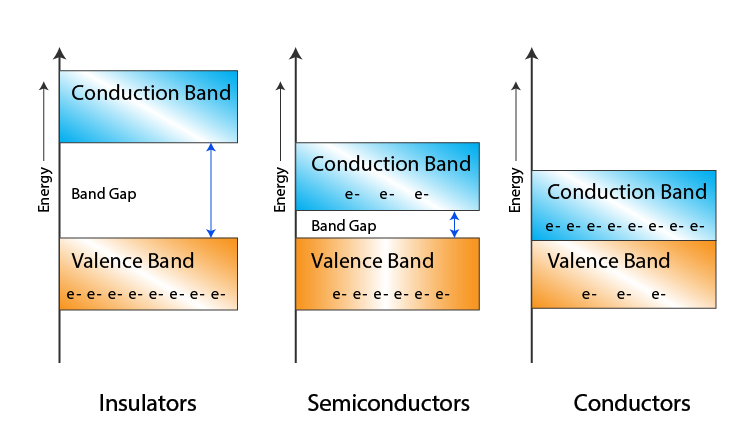
\includegraphics[width=0.7\linewidth]{img/Energy-band-diagram}
				\caption[Energy Bands]{Energy Bands}
				\label{fig:energy-band-diagram}
			\end{figure}
			
			\item Metals: $ E_G = 0 $ even at 0K. So, $ e^- $ are available even at 0K.
			\item Semiconductor: At 0K, behaves like insulator($ E_G = 1eV $). At 300K, band gap starts decreasing so conductivity increases(however, not as conductive as metals).
			\item Insulator: $ E_G = 5eV \;to\; 15 eV $ so $ e^- $ will not jump at any temp. Conductivity $\sigma = 0$ for ideal insulator; negligible practically.
			\item $ E_G \propto \dfrac{1}{temp} $
			\item $ E_{G(T)} = E_{G0} - \beta T $; ($\beta$ is $ 2.2  \times  10^{-4} $ for Ge; $ 3.6 \times  10^{-4} $ for Si)
			\item \begin{tabular}{|c|c|c|c|}
				\hline
				& Ge & Si & GaAs \\
				\hline
				$ E_{G0} $ & 0.75eV & 1.21eV & - \\
				\hline
				$ E_{G300} $ & 0.72eV & 1.1eV & 1.47eV \\
				\hline
			\end{tabular}
		\end{itemize}
		\item \textbf{Operating Temperature}: Maximum range in which the device operates. After this, melting pt. is reached and properties change. Below operating temp., band gap increases and secondary properties are seen.
			\begin{tabular}{|c|c|c|}
				\hline
				Ge & Si & GaAs \\
				\hline
				-60C to 75C & -60 to 175C & -60C to 275C \\
				\hline
			\end{tabular}
		\item \textbf{Electric Field Intensity($\epsilon$ or E)}: 
			\begin{itemize}
				\item aka field gradient
				\item $ \epsilon= \frac{dv}{dx} = $voltage/length or width
			\end{itemize}
		\item \textbf{Mobility($\mu$)}: How freely charge carriers drift(Drift $\to$ by force) in semiconductor.\\
			$\mu = \frac{Drift\; velocity(V)}{Electric\;Field\;Intensity(\epsilon)} = \frac{m^2}{V\;sec}$\\
			$\mu \propto T^{-m}$\\
			Ge: $\frac{\mu_n}{\mu_p} ~ 2.1$\\Si: $\frac{\mu_n}{\mu_p} ~ 2.6$\\
			As field intensity increases, the number of collisions decrease, therefore decreasing the mobility(fig. \ref{fig:mobility-applied-electric-field-graph}) \\
			\begin{figure}
				\centering
				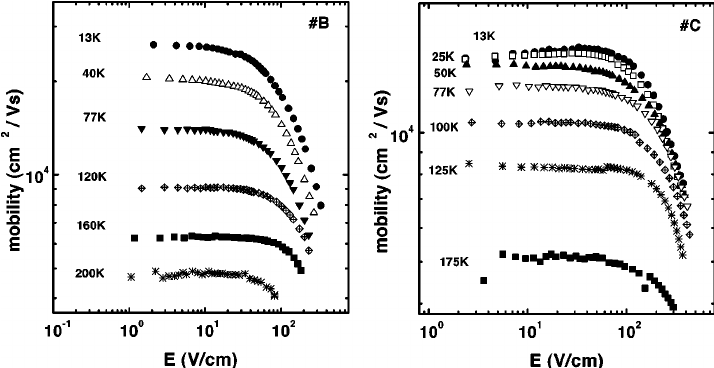
\includegraphics[width=0.7\linewidth]{img/Mobility-applied-electric-field-graph}
				\caption{graph}
				\label{fig:mobility-applied-electric-field-graph}
			\end{figure}
			\begin{tabular}{|c|c|c|c|}
				\hline
				& Ge & Si & GaAs \\
				\hline
				$\mu_n$ & $ 3800\; cm^2/V\:sec$ &  $ 1300\; cm^2/V\:sec$ &  $ 5800\; cm^2/V\:sec$ \\
				\hline
				$\mu_p$ &  $ 1800\; cm^2/V\:sec$ &  $ 500\; cm^2/V\:sec$ &  $ 400\; cm^2/V\:sec$ \\
				\hline
			\end{tabular}
			Ge is better for high freq. applications due to high Gain Bandwidth Product\\
			GaAs is best for microwave applications\\
			Si is best for switching applications.
		\item \textbf{Mass Action Law}: 
		\begin{itemize}
			\item In an extrinsic semiconductor under thermal equilibrium, the product of electrons and holes is always a constant, and is equal to the square of intrinsic concentration.
			\item $ n \times p = n_i^2 $
			\item This can be used to calculate the concentration of minority charge carriers.
			\item Therefore, $ n_p = \frac{n_i^2}{p_p} $
			\item $ majority\: carrier \propto Doping\: concentration $
		\end{itemize}
		 \item $ n_i $(Intrinsic Semiconductor Concentration):\\
		 $ n_i^2 = A_0 T^3 e^{- \frac{E_{G0}}{KT}} $, where:\\
		 $ A_0 $ is the material constant\\
		 $ T $ is the temperature\\
		 $ E_{G0} $ is the band gap
		 \item \begin{tabular}{|c|c|}
		 	\hline
		 	NTC(Negative Temp. Coeff) & PTC(Positive Temp. Coeff) \\
		 	\hline
		 	$ E_G,\ mu $ & $ n_i, v_t $ \\
		 	\hline
		 \end{tabular}
	  	 \item \textbf{Resistivity}: Specific resistance of any material($ \ohm \: m, \ohm \: cm $)\\
	  	 \begin{tabular}{|c|c|}
	  	 	\hline
	  	 	Metals & Semiconductor \\
	  	 	\hline
	  	 	Incr. with Temp. & Decr. with Temp. \\
	  	 	\hline
	  	 \end{tabular}
  	 	 \item \textbf{Conductivity}: Current carrying capacity of material($ \sigma = 1/\rho $)\\
  	 	 $\sigma = carrier\: conc \times charge \times mobility$\\
  	 	 For metals: $\sigma = n \times q \times \mu$(decreases with temp.)\\
  	 	 For semiconductors: $\sigma = nq\mu_n + pq\mu+p$ (since both $ e^- $ as well as holes contribute)(overall incr. with temp.)
  	 	 \item \textbf{Current density}: $ J = I/A \: Amp/m^2 = \sigma E $\\
  	 	 See sigma formulae from above as well
  	 	 \item \textbf{Diffusion Constant}: This a property of the material. It depends on temperature.
  	 	 \item \textbf{Diffusion Length}: The average length a carrier moves between generation and recombination. \\
  	 	 $ L = \sqrt{D\tau} $, where $\tau$ is the average lifetime\\
  	 	 $ e^- $ diffusion length $ L_n = \sqrt{D_n\tau_n} $
  	 	 \item \textbf{Concentration Gradient}: $ \frac{dn}{dx} $ is the $ e^- $ concentration gradient. $ \frac{dp}{dx} $ is holes concentration gradient.
  	 	 \item $ J_p(diff) = +q\:D_n\frac{dn}{dx}  A/cm^2$\\$ J_n(diff) = -q\:D_p\frac{dp}{dx}  A/cm^2$ \\
  	 	 $ J_{(diffusion)} = J_{n(diff)} + J_{p(diff)} $ \\
  	 	 $ I_n(diff) = J_{n(diff}) \times A $, where A is the cross sect. area\\
  	 	 Total current, $ J = J(diff) + J(drift) $ \\
   	 	 $ J_n = qD_n\frac{dn}{dx} + nQ\mu_n \epsilon $ (similar for $ j_p $)
	\end{itemize}
	\section{Einstein's Equation}
	\begin{itemize}
		\item $ \frac{D_n}{\mu_n} = V_T = kT = \frac{D_p}{\mu_p} $, where $ D $ is the Diffusion constant
		\item unit of $\frac{D}{\mu}$ is Volt
	\end{itemize}
	\section{Semiconductors}
\begin{itemize}
	\item conductivity between conductor and insulator
	\item around $ 1eV-1.5eV $
	\item Bipolar
	\item NTC
\end{itemize}
	\section{Doping}
	process of adding impurities in SC. doping $\uparrow$, carrier conc.$\uparrow$, conductivity $\sigma$$\uparrow$
	\begin{enumerate}
		\item Trivalent/Acceptor impurities: B, Al, Ge, Sn
		\item Pentavalent/Donor impurities: P, As, Sb, Bi
		\item doping is based on conc. of impurities.
		\begin{enumerate}
			\item Moderate Doping: 1/[$ 10^6 \; to\; 10^8 $] $\rightarrow$ $ P\; N $
			\item Lightly Doping: 1/[$ 10^11$] $\rightarrow$ $ P^-\; N^- $
			\item Highly Doping: 1/[$ 10^3 $] $\rightarrow$ $ P^+\; N^+ $
		\end{enumerate}
		\item 1/$ 10^8 $ converts intrinsic to extrinsic \\
		1/$ 10^8 $ doping in Ge $\rightarrow$ $\sigma$ $\uparrow$ 12 times \\
		1/$ 10^7 $ doping in Ge $\rightarrow$ $\sigma$ $\uparrow$ 120 times
		\item Doping can be homogeneous(same throughout) or non homogeneous(different at diff. points)
		\item Ge-Si crystal: intrinsic at 300K
	\end{enumerate}
	\section{Extrinsic SC}
	aka doped SC/Impurity SC/Artificial SC/degenerate SC/Compensated SC \\
	\subsection{N type or Donor SC}
	\begin{itemize}
		\item Pentavalent
		\begin{figure}[h]
			\centering
			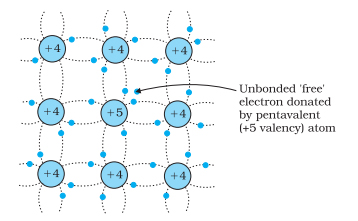
\includegraphics[width=0.7\linewidth]{img/Extrinsic-semiconductor-1}
			\caption{N-type SC}
			\label{fig:extrinsic-semiconductor}
		\end{figure}
		\begin{figure}[h]
			\centering
			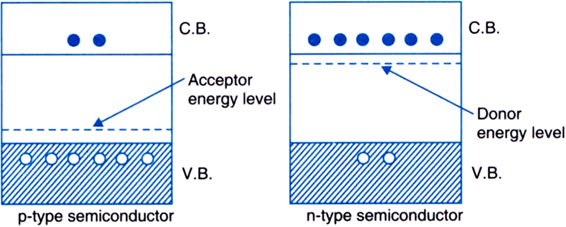
\includegraphics[width=0.7\linewidth]{img/extrinsic_band_gap}
			\caption{SC band gap at 300K \\ Donor energy lvl is 0.01 eV for Ge, 0.05 eV for Si}
			\label{fig:extrinsic-band-gap}
		\end{figure}
		\item As temp $\uparrow$ from 0K to 300K, 5th $ e^- $ move from donor lvl to conduction(fig. \ref{fig:energy-band-diagram})
		\item P type SC is represented with (+) because it has pentavalent atoms that have lost their $ e^- $
	\end{itemize}
	\subsection{P type or Acceptor SC}
	\begin{itemize}
	\item Trivalent
	\begin{figure}[h]
		\centering
		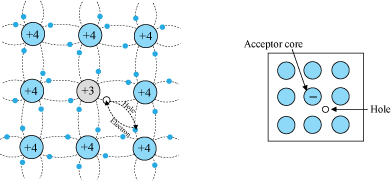
\includegraphics[width=0.7\linewidth]{img/p_type}
		\caption{P-type SC}
		\label{fig:ptype}
	\end{figure}
	
	\item See fig. \ref{fig:extrinsic-band-gap} for band gaps
	\item P type SC is represented with (+) because it has pentavalent atoms that have lost their $ e^- $
	\item Holes act as majority charge carrier. $ p>n_i $
	\item $ N_D + p = N_A + n $ \\ $ n + N_A = p $ \\ $ p \approx N_A $
	\end{itemize}
	\textbf{Q1:} Calculate the intrinsic conductivity \& intr. resistivity of Ge at 300K. $ n_i = 2.5 \times  10^{13} atoms/cm^3,\mu_n = 3800 cm^2/V\: sec, \mu_p = 1800 cm^2/V\: sec $ \\
	Ans: 
	$\sigma_i = n_i q [\mu_p + \mu_n] = 0.0222 $\\
	\textbf{Q2:} How many times $\sigma$ $\uparrow$ in the sc due to doping, IR = $ 1:10^7 $ Assume total no. of atoms = $ 4.421 \times 1-^{22} /cm^3 ; n_i = 2.5 \times 10^{13} / cm^3$\\
	Ans: 
	$ \frac{\sigma_n}{\sigma_i} = 120 times $\\
	\textbf{Q3:} A pure SC is doped with acceptor impurities to extent of 4 impurity atoms for every 1 million of atoms. calculate $\sigma$\\
	
	\chapter*{TODO}
	\section{Fermi Level}
	\subsection{In intrinsic SC:}
	In intrinsic SC, $ n = p $ \\
	$ N_c  e^{-\frac{E_c-E_F}{kT}}  = N_v e^{-\frac{E_F-E_V}{kT}}$ \\
	$ ln \frac{N_c}{N_v}  = \frac{E_c+E_v-2E_F}{kT}$ \\
	$ E_F = \frac{E_C+E_V}{2} -\frac{kT}{2}ln\frac{N_c}{N_v}$\\
	\begin{itemize}
		\item \textbf{Case-1 } Let $ m_p = m_n $(assumption) $ N_c = N_v $\\
		$ E_F = \frac{E_c + E_v}{2} $ 
		\item At T=0K, fermi lvl lies in middle of CB\&VB. Hole conc. is 0 in VB
		\item \textbf{At T=300K} $ E_F = \frac{E_c+E_v}{2} -\frac{kT}{2} ln \frac{N_c}{N_v}$ since $ N_c > _v $ and T > 0, fermi lvl will be lower. (see fig. \ref{fig:fermilvl})
		\begin{figure}
			\centering
			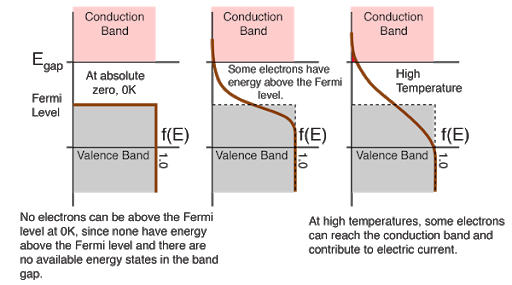
\includegraphics[width=0.7\linewidth]{img/fermi_lvl}
			\caption{}
			\label{fig:fermilvl}
		\end{figure}		
	\end{itemize}

	\subsection{In N type SC: Effect of temp.}
	$ n \approx N_D $ \\
	$ N_c  e^{-\frac{E_c-E_F}{kT}}  \approx N_D$ \\
	$ ln\frac{N_C}{N_D}  = \frac{E_C - E_F}{kT}$ \\
	$ E_F = E_C - kT\; ln \frac{N_C}{N_D} $
	\begin{itemize}
		\item \textbf{Case 1} T = 0K \\
		$ E_F = E_C $ so, no holes and no $ e^- $
		\item \textbf{At 300K} $ E_F = E_C - k T\; ln \frac{N_C}{N_D} $ \\
		see fig. \ref{fig:fermilvlntype}
		\item \textbf{At more than 300K}: $ E_C > E_F $ since $\sigma$$\downarrow$ with temp \\
		so, $ E_F $ goes downward
		\begin{figure}
			\centering
			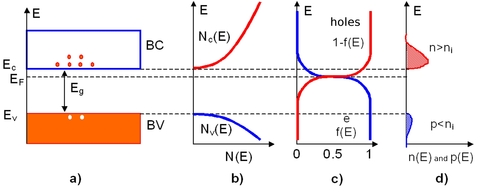
\includegraphics[width=0.7\linewidth]{img/fermi_lvl_ntype}
			\caption{}
			\label{fig:fermilvlntype}
		\end{figure}
	\end{itemize}
	\subsection{In N type SC: Effect of Doping}
	$ N_D \uparrow, let \; N_D > N_C $\\
	$ E_C < E_F $
	\begin{enumerate}
		\item \textbf{if $ N_D \approx N_C $} $ E_F = E_C $
		\item \textbf{if $ N_D > N_C $} $ E_F > E_C $
		\item \textbf{if $ N_D < N_C $} $ E_F < E_C $
	\end{enumerate}
	\subsection{In P type SC: HOMEWORK}

\end{document}